
\documentclass{article}


% \documentclass[tikz, margin=3mm]{standalone}


% \usepackage{draftwatermark}
% \SetWatermarkText{Draft}
% \SetWatermarkScale{5}
% \SetWatermarkLightness {0.9} 
% \SetWatermarkColor[rgb]{0.7,0,0}

\usepackage{geometry}                		% See geometry.pdf to learn the layout options. There are lots.
\geometry{margin=0.75in}
\geometry{letterpaper}                   		% ... or a4paper or a5paper or ... 
%\geometry{landscape}                		% Activate for for rotated page geometry
%\usepackage[parfill]{parskip}    		% Activate to begin paragraphs with an empty line rather than an indent
\usepackage{graphicx}				% Use pdf, png, jpg, or eps� with pdflatex; use eps in DVI mode
								% TeX will automatically convert eps --> pdf in pdflat						
								% TeX will automatically convert eps --> pdf in pdflatex		
\usepackage{amssymb}
\usepackage{mathrsfs}
\usepackage{hyperref}
\usepackage{url}
\usepackage{subcaption}
\usepackage{authblk}
\usepackage{amsmath}
\usepackage{amsthm}
\usepackage{mathtools}
\usepackage{graphicx}
\usepackage[export]{adjustbox}
\usepackage{hyperref}
\usepackage{alltt}
\usepackage{color}
\usepackage[utf8]{inputenc}
\usepackage[english]{babel}
\usepackage{float}
\usepackage{bigints}
\usepackage{braket}
\usepackage{siunitx}
\usepackage{setspace}
%
%	TikZ et al
%
\usepackage{tikz}
\usetikzlibrary{calc,patterns,angles,quotes,shapes,calc,intersections,decorations}    
\usepackage{tkz-euclide}
\usepackage{pgfplots}	
\usepackage{relsize}	
\usepackage{pgfplots}
%						
 %
 %
\newtheorem{thm}{Theorem}[section]
% \newtheorem{defn}[thm]{Definition}
\theoremstyle{definition}
\newtheorem{definition}{Definition}[section]
\newtheorem{proposition}{Proposition}[section]
\newtheorem{lemma}{Lemma}[section]
\newtheorem{example}{Example}[section]

\newcommand{\argmax}{\operatornamewithlimits{argmax}}
\newcommand{\argmin}{\operatornamewithlimits{argmin}}

 
\title{A Few Notes on the Principle of Least Action \\ and Newton's Second Law of Motion}
\author{David Meyer \\ dmm@1-4-5.net}

\date{Last update: \today}							% Activate to display a given date or no date


\begin{document}
\maketitle

\section{Introduction}
The principle of least action, which is also known as the stationary-action principle, is a variational principle that, when applied to the action of a mechanical system, 
amazingly yields the equations of motion for that system. The principle states that the trajectories (i.e. the solutions of the equations of motion) are stationary points of the 
system's action functional  \cite{malham2016}. One of the many amazing aspects of the principle is that it can be used to derive Newton's Second Law, Lagrangian and 
Hamiltonian equations of motion, and even  general relativity (see Einstein–Hilbert action \cite{wiki:einstein_hilbert_action}). 

\bigskip
\noindent
These notes explore a bit of the connection between the Principle of Least Action \cite{wiki:stationary_action_principle} and Newton's Second Law \cite{wiki:newtons_laws}.

\section{Finding the Minimum of a Function}
\label{sec:minimum}
{\setstretch{1.0} 
The story starts with how we use calculus to find the minimum of a function. In particular, suppose we have some function $f(x)$. We know that 
if we move a small distance from $x$, call it $\epsilon$, around $f$'s minimum\footnote{$\frac{df}{dx}= 0$ at $f$'s minimum, also known as a 
\emph{stationary point} of $f$.} then $f(x) = f(x + \epsilon)$ and so $f(x + \epsilon) - f(x) = 0$. For example consider $f(x) = x^2 +1$. This case
 is shown in Figure \ref{fig:parabola}, where we can see that $f(0) = f(0+\epsilon) = 1$ and $ \dfrac{d}{dx} f(0)  = \dfrac{d}{dx} f(0 + \epsilon) = 0$. \par}

\bigskip
\begin{figure}[H]
\centering
  \resizebox{0.75 \textwidth}{!} {                                                                                                                                                % resize figure if you want
  \begin{tikzpicture} [every edge quotes/.append style = {anchor=south, sloped}, declare function={f(\x)=\x*\x + 1;}]             % define f(x)
       \draw[thick, ->] (-5,0) -- (5,0) coordinate [label={[xshift=0.30cm, below] $x$}];                                                                 % horizontal axis
       \draw[thick, ->] (0,-1) -- (0,5) coordinate [label={[xshift=-0.30cm, left] $f(x)$}];                                                                 % xshift -- get some extra space
       \draw [line width=0.20mm, smooth,samples=100,domain=-1.75:1.75] plot (\x,{f(\x)});                                                                                     % draw f(x)
       \path (0,0) node[below left] {$O$};    
       \coordinate (p) at (0,{f(0)});                                                                                                                                                % draw a dot at minimum
       \coordinate (x) at (0,{1/(4*f(1))});                                                                                                                                        % coordinate for tangent line
       \node[very thick, circle through={(p)}] (cir) at (x) {};
       \draw[line width=0.25mm,red] (-3,{f(0)})-- (3,{f(0)});
       \fill (p)circle (0.05);                                                                                                                                                             % draw a dot at minimum (draw last to ensure it's black)
%
% draw dots on curve and axis
%
       \coordinate (e0) at (0.15,0);
       \fill (e0) circle(0.05);      
       \coordinate (e1) at (0.15,{f(0)});
       \fill (e1) circle(0.05);      
       \draw[dashed] (0.15,{f(0)}) -- (0.15,0) coordinate [label={[scale=1.10, below]  $\epsilon$}];                                            % draw epsilon under dot     
       \draw (5.5,1) node[rectangle, draw, very thin] {$\displaystyle \dfrac{d}{dx} f(x)  = \dfrac{d}{dx} f(x + \epsilon) = 0$};      % show derivatives at zero in box to the right
   \end{tikzpicture}
   }                                                                                                                                                                                             % end resizebox                                                                                           
 \caption{${\displaystyle f(x)= x^2 + 1}$}
 \label{fig:parabola}
\end{figure}



\newpage
\noindent
We also know that we can evaluate $f(x + \epsilon)$ using a Taylor series \cite{wiki:taylor}. In particular


\begin{equation*}
\begin{array}{lllll}
f(x + \epsilon)
&=&  f(x) + \epsilon \dfrac{df}{dx} + \dfrac{\epsilon^2}{2!} \dfrac{d^2 f}{dx^2} +  \dfrac{\epsilon^3}{3!}  \dfrac{d^3 f}{dx^3} + \cdots      &\qquad \mathrel{\#} \text{definition of the Taylor series for $f(x + \epsilon)$}
\end{array}
\end{equation*}

\bigskip
\noindent
Now if we define $\Delta f = f(x + \epsilon) - f(x)$ we see that

\begin{equation*}
\begin{array}{lllll}
\Delta f
&=& f(x + \epsilon) - f(x)                                                                                                                     &\qquad \mathrel{\#} \text{definition of $\Delta f$}  \\
[10pt]
&=&  \left [f(x) + \epsilon \dfrac{df}{dx} + \dfrac{\epsilon^2}{2!} \dfrac{d^2 f}{dx^2} + \dfrac{\epsilon^3}{3!} \dfrac{d^3 f}{dx^3}  + \cdots \right ]  - f(x)  
                                                                                                                                                           &\qquad \mathrel{\#} \text{substitute Taylor series for $f(x + \epsilon)$} \\
[10pt]
&=& \epsilon \dfrac{df}{dx} + \dfrac{\epsilon^2}{2!}  \dfrac{d^2 f}{dx^2} +  \text{higher order terms}  &\qquad \mathrel{\#} \text{$f(x)$ cancels} \\
[10pt]
&=& 0 + \dfrac{\epsilon^2}{2!} \dfrac{d^2 f}{dx^2} +  \cdots                                                               &\qquad \mathrel{\#} \text{$\dfrac{df}{dx} = 0$ at $f$'s minimum} \\
[10pt]
&=&  \dfrac{\epsilon^2}{2!}  \dfrac{d^2 f}{dx^2}  + \cdots                                                                   &\qquad \mathrel{\#} \text{simplify} \\
[10pt]
&\approx& \dfrac{\epsilon^2}{2!} \dfrac{d^2 f}{dx^2}                                                                                                   
                                                                                                                                                           &\qquad \mathrel{\#} \text{$\epsilon$ is close to zero so we can ignore higher order terms}
\end{array}
\end{equation*}

\bigskip
\noindent
So we can say that $\Delta f \sim \epsilon^2$, that is, the difference is a second order effect in $\epsilon$. Said from the perspective of first-order variation we can say 
that the first-order variation in the value of $f$ is constant in some neighborhood around $f$'s stationary point (that is, where the gradient of $f$ equals zero).  

\bigskip
\noindent
So in summary we know that for normal functions $f$ at the minimum

\smallskip
\begin{equation}
\Delta f =  f(x + \epsilon) - f(x)  = 0
\label{eqn:Delta}
\end{equation}

\bigskip
\noindent
at least to the first order in $\epsilon$. The constraint specified by Equation \ref{eqn:Delta} will become important when we study $\delta \mathcal{S}$.

\bigskip
\noindent
Another way to see this is that if we only consider the first order terms of the Taylor series we see that

\begin{equation*}
\begin{array}{lllll}
\Delta f 
&=&  f(x + \epsilon) - f(x)                                           &\mathrel{\#} \text{definition of $\Delta f$ (Equation \ref{eqn:Delta})} \\
[4pt]
&=& f(x) + \epsilon \dfrac{df}{dx} - f(x)                      &\mathrel{\#} \text{consider only $1^{\text{st}}$ order effects so only use the first 2 terms of the Taylor series for $f(x + \epsilon)$} \\
[4pt]
&=& \epsilon \dfrac{df}{dx}                                        &\mathrel{\#} \text{$f(x)$ cancels} \\
[4pt]
&=& 0                                                                        &\mathrel{\#} \text{$\dfrac{df}{dx} = 0$ at the extremums \cite{wiki:extremum}} \\
\end{array}
\end{equation*}

\bigskip
\noindent
So we can see that $\Delta f$ must equal zero, at least to the first order in $\epsilon$.


\bigskip
{\setstretch{1.55}
\noindent
An important (or maybe, the most important) difference between the approach taken by the Principle of Least Action and Newton's Second Law is that the Principle 
of Least Action looks at the value of an entire  \emph{path}, where as Newton's Second Law looks at points along the path. That is, the Newtonian approach is local
while the Principle of Least Action approach is global. More specifically, in Newton's case we 
are given initial conditions (the initial position and the initial velocity) and then solve the differential equation ($F=ma$) for $x(t)$. Put another way,
in Newtonian mechanics we  solve $- \dfrac{\partial V}{\partial x} = m \dfrac{d^2x}{dt^2}$ to find $x(t)$. As we will see in Section
\ref{sec:pola}, Lagrangian mechanics takes a different approach: we find an object's trajectory $x(t)$ from its beginning 
and ending positions (the boundary values). Amazingly these two approaches turn out to be equivalent. \par}

\section{The Principle of Least Action}
\label{sec:pola}
The action, denoted $\mathcal{S}$,  is defined to be the sum of the difference between a particle's kinetic energy \cite{wiki:kinetic_energy} and its potential energy \cite{wiki:potential_energy} at every 
point along its path.  $\mathcal{S}$ is just a number that is associated with the trajectory (path).  The Principle of Least  Action states that the path for which the sum of these differences (that is,  
$\mathcal{S}$) is minimum is the actual path the particle will take. To show that this is the case all of the proofs that I have seen rely on the fact that the Principle of Least  Action and Newton's 
Second Law ($F=ma$) are equivalent. These notes show this result below.

\bigskip
\noindent
To give a bit more formal definition of the Principle of Least  Action:

\medskip
\begin{definition}
{\bf The Principle of Least (Stationary) Action}: The path of a particle is the one that yields a stationary value of the action.
A stationary point of some function is a point where its gradient is equal to zero. In other words, the first-order variation in the 
value of the function is constant in some neighborhood around the stationary point. As we will see below, this condition can be
expressed as $\delta \mathcal{S} = 0$.
\end{definition}

\bigskip
\noindent
Consider the setup shown in Figure \ref{fig:pola} and imagine that the actual path is represented by the function $x(t)$. That is, $x(t)$ represents
the path of a particle that starts out at position $x_1$ at time $t_1$ and ends up at $x_2$ at time $t_2$. Then what we want to do is to look at 
another path that is some small deviation away from $x(t)$ (we know from Equation \ref{eqn:Delta} that this will be close to $x(t)$). We hope that if 
we look at the change in the action of the path with the small deviation that change should be close to zero as well.

\bigskip
\noindent
As we can see from Figure \ref{fig:pola} we call the small deviation $\eta(t)$ and we call the deviated path $x(t) + \eta(t)$. 

% Now recall
% that the action $\mathcal{S}$ is defined at the time integral from $t_1$ to $t_2$, that is
%
% \bigskip
% \begin{equation}
% \mathcal{S} = \int_{t_1}^{t_2} (KE - PE) \; dt
% \label{eqn:S}
% \end{equation}


\bigskip
\begin{figure}[H]
\centering
  \resizebox{0.60 \textwidth}{!} {                                                                                                                                                 % resize figure if you want
    \begin{tikzpicture}  [every edge quotes/.append style = {anchor=south, sloped}]
       \draw[thick, ->] (-0.35,0) -- (13.5,0) coordinate [label={[xshift=0.30cm, below]  $t$}] (t);                                                        % xshift -- get some extra space
       \draw[thick, ->] (0,-0.35) -- (0,10.5) coordinate [label={[xshift=-0.30cm, left]  $x$}] (x);                                                          % xshift -- get some extra space
       \coordinate[label=below left:$ O $] (O); 
%
% draw legend
%        
       \draw (7,8) node[right,rectangle] {$x(t)$}; 
       \draw [very thick] (9,8) -- (11,8);
       \draw (7,7)  node [right,rectangle] {${x(t) + \eta(t)}$};
       \draw [very thick,red,dashed] (9,7) -- (11,7);

%
% make some coordinates for later use
%
       \coordinate (x2) at (0,5);
       \coordinate (x1) at (0,2);
       \coordinate (t2) at (6,0);
       \coordinate (t1) at (2,0);
       \coordinate (t1x1) at (2,2);
       \coordinate (t2x2) at (6,5);
         
       \draw[draw=none] (x2) node[left] {$x(t_2)$};
       \draw [] (t2) node[below] {$t_2$};
       \draw[draw=none] (x1) node[left] {$x(t_1)$};     
       \draw[draw=none] (t1) node[below] {$t_1$};    
%
% draw points
%
         \fill (x2) circle(0.05);      
         \fill (x1) circle(0.05);                                                                                                                                                   % draw dots on axes
         \fill (t2) circle(0.05); 
         \fill (t1) circle(0.05);  
         \fill (t1x1) circle(0.05);   
         \fill (t2x2) circle(0.05);       
         
%
% the coordinates of the parabolas are unfortunately pretty much eyeballed
%
         
        \draw[yshift=-2cm, very thick,black] (2, 4) parabola[bend={+(0, 3)}, bend pos=0.5] (6, 7);                                       % draw parabolas
        \draw[yshift=-2cm, dashed, very thick,red] (2, 4) parabola[bend={+(0, 5)}, bend pos=0.5] (6, 7);     
        \coordinate (p1) at (4,6.5);                                                                                                                                         % coordinates on curves 
        \coordinate (p2) at (4,8.5);
        \draw[dashed,thick, <->] (p1) -- (p2) coordinate [label={[midway, right]  $\eta(t)$}];                                                 % draw \eta(t) between curves                                                                              
      
 %
 % draw the S integral in a box to the right
 %        
       \draw (9.5,2.25) node[draw,very thin,rectangle] {$\mathlarger {\mathlarger {{\displaystyle \; \mathcal{S} \big [ (x(t) \big ]= \int_{t_1}^{t_2} (KE - PE) \; dt \;}}}$}; 
    \end{tikzpicture}
  }                                                                                                                                                                                             % end resizebox                                                                                           
 \caption{Principle of Least Action Setup}
 \label{fig:pola}
\end{figure}

\bigskip
\noindent
Now, consider a particle moving in one dimension in a uniform gravitational field $g$ with potential energy $V(x)$\footnote{$V(x)$ is sometimes called $U(x)$, 
and is also informally referred to as $PE$.}. In this case $V(x) = m g x$. So


\begin{equation*}
\begin{array}{lllll}
\mathcal{S}\big [ (x(t) \big ]
&=& {\displaystyle \mathlarger {\int_{t_1}^{t_2}} (KE - PE) \; dt}           &\qquad \qquad \qquad \qquad \mathrel{\#} \text{definition of $\mathcal{S}\big [ (x(t) \big ]$}  \\
[14pt]
&=& {\displaystyle \mathlarger{ \int_{t_1}^{t_2}} \left [ \frac{1}{2} m \left ( \dfrac{dx}{dt} \right)^2 - V(x) \right  ] dt}   
                                                                                                              &\qquad \qquad \qquad \qquad \mathrel{\#}  KE = \frac{1}{2} m \left ( \dfrac{dx}{dt}\right )^2\!\!\!\!, \; PE = V(x)
\end{array}
\end{equation*}


\bigskip
\noindent
Note that $\mathcal{S}$ is a \emph{functional} \cite{cov} so we use square brackets (e.g. $\mathcal{S}[x(t)]$) instead of parenthesis to distinguish the functional
from the function (e.g $S(x)$). Now, abbreviating $x(t)$ by $x$ we see that

\bigskip
\begin{equation}
\mathcal{S}[x] = {\displaystyle \mathlarger{ \int_{t_1}^{t_2}} \left [ \frac{1}{2} m \left ( \dfrac{dx}{dt} \right )^2 - V(x) \right  ] dt}  
\label{eqn:S(x)}
\end{equation}


\bigskip
\noindent
Now define $\delta \mathcal{S} = \mathcal{S}[x + \eta] - \mathcal{S}[x]$. We know that the path taken by the system, $x(t)$,  has a stationary action ($\delta \mathcal{S} = 0$) 
under small changes to the configuration of the system. Said another way, we know that $\delta \mathcal{S} = 0$ to the first order in $\eta$ (here again $x$ is shorthand for $x(t)$ 
and $\eta$ is shorthand for $\eta(t)$).  So now we can expand $\mathcal{S}[x + \eta]$ as follows:


\bigskip
\begin{equation}
\begin{array}{lllll}
\mathcal{S}[x + \eta]
&=& {\displaystyle \mathlarger{ \int_{t_1}^{t_2}} \left [ \frac{1}{2} m \left ( \dfrac{d}{dt} (x+\eta) \right )^2 - V(x+\eta) \right  ] dt}   &\qquad \qquad \mathrel{\#} \text{substitute $x + \eta$ for $x$}  \\
[14pt]
&=& {\displaystyle \mathlarger{ \int_{t_1}^{t_2}} \left [ \frac{1}{2} m \left ( \dfrac{dx}{dt} + \dfrac{d\eta}{dt} \right )^2 - V(x+\eta) \right  ] dt}   &\qquad  \qquad \mathrel{\#} \text{derivative is a linear operator} 
\end{array}
\label{eqn:s_x_plus_eta}
\end{equation}

\bigskip
\noindent
Next notice that 


\bigskip
\begin{equation*}
\begin{array}{lllll}
 \left ( \dfrac{dx}{dt} + \dfrac{d\eta}{dt} \right )^2 
&=&  \left (\dfrac{dx}{dt} \right)^2 + \left (\dfrac{d\eta }{dt} \right)^2  +2 \left ( \dfrac{dx}{dt} \right ) \left ( \dfrac{d\eta}{dt} \right )          &\qquad \mathrel{\#} \text{multiply out} \\
[12pt]
&=&  \left (\dfrac{dx}{dt} \right)^2 + 2 \left ( \dfrac{dx}{dt} \right ) \left ( \dfrac{d\eta}{dt} \right )                                                              
                                                                                                                                        &\qquad \mathrel {\#} \text{$\left ( \dfrac{d\eta }{dt} \right )^2 \approx 0$ (Section \ref{sec:minimum})}
\end{array}
\end{equation*}

\bigskip
\noindent
Next want to expand $ V(x + \eta)$ using a Taylor series:

\medskip
\begin{equation*}
\begin{array}{lllll}
 V(x + \eta)
&=& V(x) + \eta \dfrac{dV}{dx} + \dfrac{\eta^2}{2!}  \dfrac{d^2V}{dx^2} + \cdots     &\quad \qquad \qquad \mathrel{\#} \text{expand Taylor series} \\
\end{array}
\end{equation*}

\bigskip
\noindent
So now if we substitute these last two expressions into Equation \ref{eqn:s_x_plus_eta}  and group terms we see that

\bigskip
\bigskip
\begin{equation*}
\begin{array}{lllll}
\mathcal{S}[x + \eta]
&=& {\displaystyle \mathlarger{ \int_{t_1}^{t_2}} \left [ \frac{1}{2} m \left ( \dfrac{dx}{dt} \right )^2 - V(x) 
+ \dfrac{1}{2} m \left (2 \dfrac{dx}{dt} \dfrac{d \eta}{dt} \right ) - \eta \dfrac{dV}{dx} - \text{higher order terms}  \right ] dt} 
\end{array}
\end{equation*}

\bigskip
\noindent
We also have the constraint that

\bigskip
\begin{equation*}
\delta \mathcal{S} = \mathcal{S}[x+\eta] - \mathcal{S}[x] = 0
\end{equation*}

\bigskip
\noindent
and we saw earlier (Equation \ref{eqn:S(x)}) that

\begin{equation*}
\mathcal{S}[x] = {\displaystyle \mathlarger{ \int_{t_1}^{t_2}} \left [ \frac{1}{2} m \left ( \dfrac{dx}{dt} \right )^2 - V(x) \right  ] dt}   
\end{equation*}


\bigskip
\noindent
Putting the last three equations together (and ignoring higher order terms in the Taylor series for $\mathcal{S}(x+\eta)$) we find that

\bigskip
\begin{equation*}
\delta \mathcal{S} =  {\displaystyle \mathlarger{ \int_{t_1}^{t_2}}  
\left [  m \left (\dfrac{dx}{dt} \dfrac{d \eta}{dt} \right ) - \eta \dfrac{dV}{dx} \right ] dt }  = 0
\end{equation*}

\medskip
\bigskip
\noindent
What we would like is to have this integral be zero regardless of the value of $\eta$. So how can we "factor out" $\eta$? The first thing to notice is that
by the product rule \cite{wiki:product_rule} we have

\begin{equation*}
\begin{array}{lllll}
\dfrac{d}{dx} \left ( \dfrac{dx}{dt} \cdot \eta \right ) 
&=&  \dfrac{d^2x}{dt^2} \cdot  \eta + \dfrac{dx}{dt} \cdot \dfrac{d \eta}{dt}                                
                                                                                                                               &\qquad  \mathrel{\#} \text{product rule: ${\displaystyle {\dfrac {d}{dx}}(u\cdot v)={\dfrac {du}{dx}}\cdot v+u\cdot {\dfrac {dv}{dx}}}$}\\
[12pt]
&\Rightarrow&  \dfrac{dx}{dt} \dfrac{d \eta}{dt} \ = \dfrac{d}{dx} \left ( \dfrac{dx}{dt} \eta \right )  - \dfrac{d^2x}{dt^2} \eta 
                                                                                                                               &\qquad  \mathrel{\#} \text{solve for $\dfrac{dx}{dt} \dfrac{d \eta}{dt}$} \\
[12pt]
&\Rightarrow& {\displaystyle  \int_{t_1}^{t_2} \dfrac{dx}{dt} \dfrac{d \eta}{dt} \ =  \int_{t_1}^{t_2} \dfrac{d}{dx} \left ( \dfrac{dx}{dt} \eta \right ) dt   - \int_{t_1}^{t_2}  \dfrac{d^2x}{dt^2} \eta \; dt } 
                                                                                                                                &\qquad \mathrel{\#} \text{integrate both sides} \\
[12pt]
&\Rightarrow& {\displaystyle  \int_{t_1}^{t_2} \dfrac{dx}{dt} \dfrac{d \eta}{dt} \ =  \dfrac{dx}{dt} \eta \bigg |^{t_2}_{t_1} - \int_{t_1}^{t_2}  \dfrac{d^2x}{dt^2} \eta \; dt } 
                                                                                                                                 &\qquad \mathrel{\#} \text{integral \& derivative in $1^{st}$ term cancel} \\
[12pt]
&\Rightarrow& {\displaystyle  \int_{t_1}^{t_2} \dfrac{dx}{dt} \dfrac{d \eta}{dt} \ =   - \int_{t_1}^{t_2}  \dfrac{d^2x}{dt^2} \eta \; dt }                   
                                                                                                                               &\qquad \mathrel{\#} \text{$\eta(t_1) = \eta(t_2) = 0$ (by definition)}
\end{array}
\end{equation*}

\bigskip
\noindent
So now we know that

\begin{equation}
 {\displaystyle  \int_{t_1}^{t_2} \dfrac{dx}{dt} \dfrac{d \eta}{dt} \ =   - \int_{t_1}^{t_2}  \dfrac{d^2x}{dt^2} \eta \; dt }  
 \label{eqn:intermediate}
\end{equation}

\bigskip
\noindent
and we saw earlier that 

\begin{equation}
\delta \mathcal{S} =  {\displaystyle \mathlarger{ \int_{t_1}^{t_2}}  
\left [  m \left (\dfrac{dx}{dt} \dfrac{d \eta}{dt} \right ) - \dfrac{dV}{dx} \eta  \right ] dt }  = 0
\label{eqn:prod}
\end{equation}

\bigskip
\noindent
so

\begin{equation*}
\begin{array}{lllll}
\delta \mathcal{S} 
&=&  {\displaystyle \mathlarger{ \int_{t_1}^{t_2}}   \left [  - m \dfrac{d^2x}{dt^2} \eta - \dfrac{dV}{dx} \eta \right ] dt }            &\qquad \mathrel{\#} \text{substitute result from Equation \ref{eqn:intermediate} into Equation \ref{eqn:prod}} \\
[12pt]
&=&  {\displaystyle \mathlarger{ \int_{t_1}^{t_2}}   \left [  - m \dfrac{d^2x}{dt^2} -  \dfrac{dV}{dx} \right ] \eta \; dt }                &\qquad \mathrel{\#} \text{factor out $\eta$} 
\end{array}
\end{equation*}

\bigskip
\noindent
Since $\delta \mathcal{S}$ must equal zero (Equation \ref{eqn:prod}) and we know $\eta(t)$ is not the constant function 0 so it must be that

\bigskip
\begin{equation*}
- m \dfrac{d^2x}{dt^2} -  \dfrac{dV}{dx} = 0
\end{equation*}


\bigskip
\noindent
But now notice that 

\begin{equation*}
 -  \dfrac{dV}{dx} =  m \dfrac{d^2x}{dt^2}
\end{equation*}

\bigskip
\noindent
and since ${\displaystyle -  \dfrac{dV}{dx} = F}$ and ${\displaystyle  \dfrac{d^2x}{dt^2} = a}$ we amazingly have arrived at Newton's Second Law \cite{wiki:newtons_laws}:

\bigskip
\begin{equation*}
F = ma
\end{equation*}

\bigskip
\noindent
Finally, in the general case we write the action $\mathcal{S}$ as

\bigskip
\begin{equation*}
\mathcal{S} \equiv \int_{t_1}^{t_2} L(x,\dot{x},t) \, dt
\end{equation*}

\bigskip
{\setstretch{1.5}
\noindent
 where $L$ is called the \emph{Lagrangian} (which we will discuss in more detail in Section \ref{sec:euler_lagrange}) and 
 $\dot{x}$ is shorthand for $\dfrac{dx}{dt}$. One other detail: the variable $x$ here can refer to any number of coordinates,
 the so-called \emph{generalized coordinates}, the $i^{th}$ of which is conventionally denoted  $q_i$. \par }




\section{The Euler-Lagrange Equation}
\label{sec:euler_lagrange}
Consider the following seemingly counter-intuitive combination of the kinetic and potential energies ($T$ and $V$ respectively):

\begin{equation}
L \equiv T  - V
\label{eqn:lagrangian}
\end{equation}


{\setstretch{1.35} 
\noindent
$L$ here is the Lagrangian.  The Lagrangian is essentially the action per unit time and as we saw above,  in classical mechanics this particular 
Lagrangian ($L = T - V$) is precisely the Lagrangian that generates Newton’s second law ($F = ma$). Next we'll briefly look at an application of the Lagrangian
which involves a simple harmonic oscillator, specifically a mass on the end of a spring. We will study this problem in a bit more detail in 
Section \ref{sec:simple_harmonic_oscillator}. \par}

\bigskip
\noindent
Here the kinetic energy $T$ is $\frac{1}{2} m \dot{x}^2$ and the spring potential energy $V,$ given by Hooke's Law \cite{wiki:hookes_law}, 
is $\frac{1}{2} k x^2$. So the Lagrangian for this case is


\bigskip
\begin{equation}
L = \dfrac{1}{2} m \dot{x}^2 - \dfrac{1}{2} k x^2
\label{eqn:moeos}
\end{equation}

\bigskip
\noindent
We need one more piece of the puzzle before we can solve for $x$ as a function of time, the  \emph{Euler-Lagrange} equation:

\bigskip
\begin{equation}
\dfrac{d}{dt} \left ( \dfrac{\partial L}{\partial \dot{x}} \right ) -  \dfrac{\partial L}{\partial x} = 0
\label{eqn:euler-lagrange}
\end{equation}

\bigskip
\noindent
Essentially the Euler-Lagrange equation is a constraint that the Lagrangian must satisfy in order for the principle of stationary action to be true. It is essentially what 
generates the equations of motion of a system given a specific Lagrangian, just as Newton’s second law does for a given set of forces.


\bigskip
{\setstretch{1.35} 
\noindent
Now, for the mass on the end of a spring problem we looked at above we can see 
that from Equation \ref{eqn:moeos} that $\frac{\partial L}{\partial \dot{x}} = m\dot{x}$, $\frac{d}{d t}  m\dot{x} = m\ddot{x}$ and $\frac{\partial L}{\partial x} = - $. Combining these results in 
Equation \ref{eqn:euler-lagrange} gives us \par}


\begin{equation*}
m \ddot{x} = -kx
\end{equation*}

\bigskip
\noindent
which is exactly the result obtained by using $F = ma$. An equation such as Equation \ref{eqn:euler-lagrange} which is derived from the Euler-Lagrange equation is called an 
equation of motion\footnote{AFAICT the term “equation of motion” is somewhat ambiguous. It is understood to refer to the second-order differential equation satisfied by $x$ 
and not the actual equation for $x$ as a function of $t$, namely $x(t) = A \cos(\omega t + \phi)$ in this problem, which is obtained by integrating the equation of motion twice.}.

\bigskip
\noindent
I'll just note here that this Lagrangian is frequently written like this:

\begin{equation*}
L = \dfrac{1}{2} m \dot{x}^2 - V(x)
\end{equation*}

\bigskip
\noindent
The integral of $L$ between two points $t_1$ and $t_2$ gives us the \emph{action} of the path between those points (Equation \ref{eqn:S(x)}).

\bigskip
\noindent
Now, if we combine the Lagrangian (Equation \ref{eqn:lagrangian}) with the Euler-Lagrange equation (Equation \ref{eqn:euler-lagrange}) we get


\begin{equation*}
m \ddot{x} = - \dfrac{d V} {d x}
\end{equation*}

\bigskip
\noindent
But  $- \frac{dV}{dx}$ is just the force on the particle. So as we saw at the end of Section \ref{sec:pola}
Equations \ref{eqn:lagrangian} and \ref{eqn:euler-lagrange} (albeit written in different notation) together again 
tell us that $F = ma$.

\section{A Bit More Detail on the Simple Harmonic Oscillator Problem}
\label{sec:simple_harmonic_oscillator}
In Section \ref{sec:euler_lagrange} we briefly considered the dynamics of a mass on the end of a spring and 
introduced the Euler-Lagrange equation (Equation \ref{eqn:euler-lagrange}) as a method to solve the system. 
In this section we'll consider this problem in a bit more detail and use the Euler–Lagrange equation to solve 
for the position of the mass as a function of time. 

\bigskip
\noindent
To start, consider the simple harmonic oscillator \cite{wiki:harmonic_oscillator} 
shown in Figure \ref{fig:shm}. Here the mass $m$ is moving back and forth in one dimension on a frictionless surface with 
spring constant $k$ and equilibrium point EP.


\begin{figure}[H]
\centering
  \resizebox{0.65 \textwidth}{!} {                                                                                                                                                           % resize figure if you want
   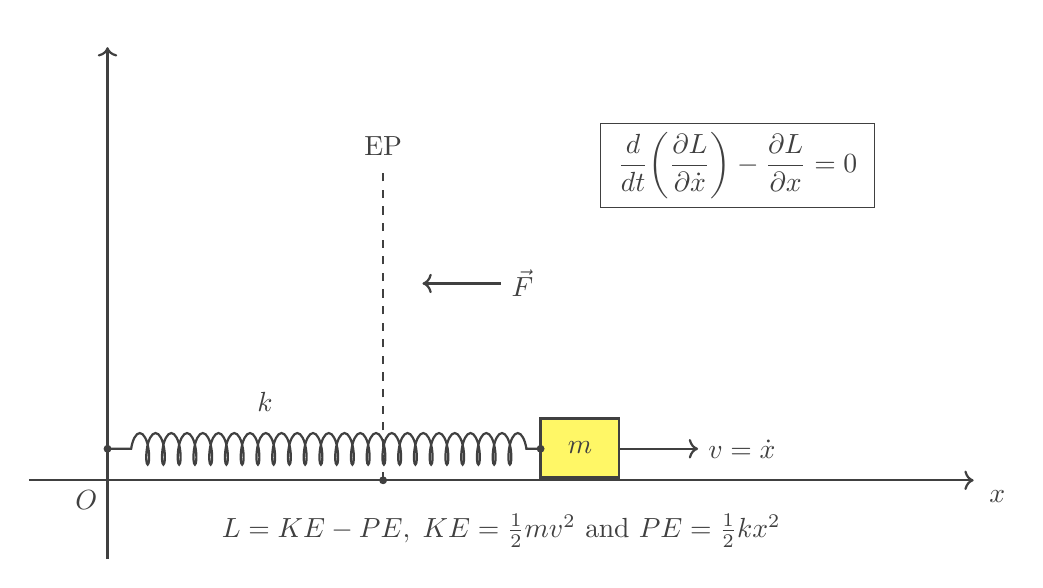
\begin{tikzpicture}[black!75,thick]
        \draw[thick, ->] (-1,0) -- (11,0) coordinate [label={[xshift=0.30cm, below] $x$}];                                                                          % horizontal axis
        \draw[thick, ->] (0,-1) -- (0,5.5) coordinate [label={[]}];                                                                                                                 % xshift -- get some extra space
        \draw[draw=none] (-1,0) -- (11,0) coordinate [label={[yshift=-0.3cm,midway,below] 
                                      ${L = KE- PE, \; KE = \frac{1}{2} m v^2  \text{ and } PE = \frac{1}{2} k x^2}$}];                                             % draw the equations below the x axis
        \draw (8,4) node[rectangle, draw, very thin] 
                         {$\mathlarger {\; \dfrac{d}{dt} \bigg ( \dfrac{\partial L}{\partial \dot{x}} \bigg ) - \dfrac{\partial L}{\partial x} = 0 \;}$};    % draw the Euler-Lagrange equation to the right
       \path (0,0) node[below left] {$O$};    

%
% draw the spring 
%
        \draw [
              decoration={
                 coil,
                 aspect=0.3, 
                 segment length=2mm, 
                 amplitude=2mm, 
                 pre length=3mm,
                 post length=3mm},
             decorate] (0,0.40) -- (5.75,0.40);
        \fill (0,0.40) circle(0.05);                                                                                                                                                                 % draw a dot connecting the spring to the y axis

 %
 % draw the mass
 %
       \node[draw,
	     fill=yellow!60,
	     minimum width=1cm,
	     minimum height=0.75cm,
	     anchor=north,
	     label=center:$m$] at (6,0.80) {};
      \fill (5.5,0.40) circle(0.05);                                                                                                                                                                 % draw a dot connecting the mass to the spring
       
      \draw[->] (6.5,0.40)-- (7.5,0.40) coordinate [label={[right] ${v = \dot{x}}$}];                                                                                      % draw velocity vector (v) to the right of the mass
      
%
% other annotation of axes etc
%
      \coordinate (k) at (2,1.25);
      \draw[draw=none] (k) node[below] {$k$};    
      \coordinate (c1) at (3.5,0);
      \coordinate (c2) at (3.5,4);
      \coordinate (c3) at (3.5,2.5);
      \coordinate (c4) at (6,2.5);
      \draw[dashed] (c1) -- (c2) coordinate [label={[above] EP}];   
      \draw[<-] (4,2.5) -- (5,2.5) coordinate [label={[right] $\vec{F}$}];   
      \fill (c1) circle(0.05);      
    %  \fill (c3) circle(0.05);      
    \end{tikzpicture}
  }                                                                                                                                                                                                                     % end resizebox                                                                                           
\caption{Simple Harmonic Oscillator Setup}
\label{fig:shm}
\end{figure}


\noindent
In this example we will be using generalized coordinates so we use $v = \dot{x}$ and write the kinetic energy $KE = \dfrac{1}{2} m \dot{x}^2$. So we can
write the Lagrangian as follows:

\bigskip
\begin{equation*}
L = KE - PE = \dfrac{1}{2} m \dot{x}^2 - \dfrac{1}{2} k x^2
\end{equation*}


\bigskip
\noindent
To find the position of the mass $m$ as a function of time (call it $x(t)$) we need to solve the Euler–Lagrange equation for this value of $L$. Recall that 
the  Euler–Lagrange equation is


\bigskip
\begin{equation*}
\dfrac{d}{dt} \left ( \dfrac{\partial L}{\partial \dot{x}} \right ) -  \dfrac{\partial L}{\partial x} = 0
\end{equation*}

\bigskip
\noindent
So first we want to compute $\dfrac{\partial L}{\partial x} = \dfrac{\partial}{\partial x}  \bigg [ \dfrac{1}{2} m \dot{x}^2  - \dfrac{1}{2} k x^2 \bigg ]$. 
Since differentiation is a linear operation \cite{wiki:linearity_of_differentiation} and we know that 
$\dfrac{\partial}{\partial x} \bigg [\dfrac{1}{2} m \dot{x}^2  \bigg ] = 0$ we can see that 

\bigskip
\begin{equation*}
\dfrac{\partial L}{\partial x} = \dfrac{\partial}{\partial x}  \bigg [ \dfrac{1}{2} m \dot{x}^2  - \dfrac{1}{2} k x^2 \bigg ] 
= \dfrac{\partial}{\partial x} \bigg [\dfrac{1}{2} m \dot{x}^2  \bigg ] - \dfrac{\partial}{\partial x} \bigg [\dfrac{1}{2} k x^2  \bigg ]  
=  0 - \dfrac{\partial}{\partial x} \bigg [\dfrac{1}{2} k x^2  \bigg ] 
= - \dfrac{\partial}{\partial x} \bigg [ \dfrac{1}{2} k x^2  \bigg ]  
= - \dfrac{1}{2} 2 k x = -kx
\end{equation*}

\bigskip
\noindent
Next, we want to find  $\dfrac{\partial L}{\partial \dot{x}}$ and then take its derivative with respect to $t$ (time). Here we know that 
$\dfrac{\partial}{\partial \dot{x}} \Bigg [ \dfrac{1}{2} k x^2 \Bigg ] = 0$ and so


\begin{equation*}
\dfrac{\partial L}{\partial \dot{x}} = \dfrac{\partial}{\partial \dot{x}} \Bigg [   \dfrac{1}{2} m \dot{x}^2 - \dfrac{1}{2} k x^2 \Bigg ] 
= \dfrac{\partial}{\partial \dot{x}} \Bigg [ \dfrac{1}{2} m \dot{x}^2 \Bigg ] - \dfrac{\partial}{\partial \dot{x}} \Bigg [  \dfrac{1}{2} k x^2 \Bigg ] 
= \dfrac{\partial}{\partial \dot{x}} \Bigg [  \dfrac{1}{2} m \dot{x}^2 \Bigg ]  - 0
= \dfrac{\partial}{\partial \dot{x}} \Bigg [  \dfrac{1}{2} m \dot{x}^2 \Bigg ] =  \dfrac{1}{2} 2 m \dot{x} = m \dot{x}
\end{equation*}

\bigskip
\noindent
Now we can see that $\dfrac{d}{dt} \bigg ( \dfrac{\partial L}{\partial \dot{x}} \bigg )   = \dfrac{d}{dt} \big ( m \dot{x} \big ) = m \ddot{x}$. Plugging these values back into the 
Euler–Lagrange equation we find that

\bigskip
\begin{equation*}
\dfrac{d}{dt} \bigg ( \dfrac{\partial L}{\partial \dot{x}} \bigg ) - \dfrac{\partial L}{\partial x} = m \ddot{x} - (-kx) = m \ddot{x} + kx \Rightarrow \ddot{x} + \dfrac{k}{m} x = 0
\end{equation*}

\bigskip
{\setstretch{1.80}
\noindent
Here we recognize that $\ddot{x} + \dfrac{k}{m} x = 0$ is a differential equation that has a solution in sine or cosine (doesn't matter which) where $\dfrac{k}{m}$ represents
 the angular frequency. If we let $\omega_0 = \sqrt{\dfrac{k}{m}}$ then $\omega_0^2 = \dfrac{k}{m}$ and so $\ddot{x} + \omega_0^2 x = 0$. But this 
 is a differential equation that has the general solution \cite{harmonic_oscillartors} \par}

 \bigskip
 \begin{equation*}
 x(t) = A \cos (\omega_0 t - \phi)
 \end{equation*}
 
 
 \bigskip
 \noindent
 where $A$ is the amplitude, $\omega_0$ is the angular frequency and $\phi$ is phase. Note that $A$ and $\phi$ depend on initial conditions while  $\omega_0$ 
 does not. 
 
 \bigskip
 \noindent
 So in this simple system the position of the mass as a function of time is given by $ x(t) = A \cos (\omega_0 t - \phi)$ for some amplitude $A$ and where the angular frequency 
 is given by the spring constant ($k$) divided by the mass of the object ($m$).

\section{Conclusions}
It's amazing that two such different approaches, Newtonian mechanics and Lagrangian mechanics, turn out to be equivalent. BTW, Kenneth Young has a nice video on the Principle
of Least Action \cite{youtube:kenneth_young_pola}.

% \newpage
\bibliographystyle{plain}
\bibliography{/Users/dmm/papers/bib/qc}
\end{document} 

